% !TEX root = ../../buch.tex
% main.tex -- Paper zum Thema <burgers>
%
% (c) 2020 Hochschule Rapperswil
%
\chapter{Die Gleichung von Burgers\label{chapter:burgers}}
\lhead{Burgers-Gleichung}
\begin{refsection}
\chapterauthor{Michael Schmid}
\index{Schmid, Michael}%
\index{Gleichung von Burgers}%

%
% einleitung.tex -- Beispiel-File für die Einleitung
%
% (c) 2020 Prof Dr Andreas Müller, Hochschule Rapperswil
%
\section{Einleitung\label{quadratur:section:einleitung}}
\rhead{Einleitung}

Im Kapitel~\ref{chapter:integration}, Integration, wurden die 
Trapezregel und die Mittelpunktsregel für die numerische Integration, 
\index{numerische Integration}%
\index{Integration, numerische}%
auch Quadratur genannt, erklärt. 
\index{Quadratur}%
In diesem Kapitel wird eine weitere Methode, die Gauss-Quadratur, erarbeitet.
Die Gauss-Quadratur ist ein Verfahren, welches ein bestimmtes Integral der Form
\index{Gauss-Quadratur}%
\begin{equation}
    \int_{a}^{b} f(x) \,dx
\end{equation}
mit der approximierten Summenformel
\index{Summenformel}
\begin{equation} \label{quadratur:equation:quadraturapproxsumme}
    I = \sum_{i=0}^{n} A_i f(x_i)
\end{equation}
annähert, wobei die Stützstellen $x_i$ und die Gewichtung $A_i$ von der gewählten 
Methode abhängen. 
Es werden dabei im Vergleich mit ähnlichen Verfahren viel weniger Funktionsauswertungen benötigt.

Methoden für die Quadratur lassen sich in zwei Gruppen unterteilen: 
Newton-Cotes-Formeln und Gauss-Quadratur.
\index{Newton-Cotes-Formel}
Die im Kapitel \ref{buch:subsection:mittelpunkt} und \ref{buch:subsection:trapez} beschriebenen
Trapezregel und Mittelpunktsregel gehören zu der ersten Kategorie.
\index{Trapezregel}%
\index{Mittelpunktsregel}%
Newton-Cotes-Formeln lassen sich dadurch erkennen, dass die Stützstellen auf der $x$-Achse 
gleichmässig verteilt sind und eignen sich besonders für die Integration, wenn sich $f(x)$ 
effizient in kleinen Intervallen berechnen lässt oder bereits von Computern berechnet worden ist.








%
% problemstellung.tex -- Beispiel-File für die Beschreibung des Problems
%
% (c) 2020 Prof Dr Andreas Müller, Hochschule Rapperswil
%
\section{Numerische Probleme des Gram-Schmidt-Verfahrens
\label{qr:section:problemstellung}}
\rhead{Problemstellung}
\index{Gram-Schmidt-Verfahren}%
In Abschnitt \ref{buch:subsection:gram-schmidt} wurde das Gram-Schmidt-Orthonormalisierungsverfahren vorgestellt.
Es liefert zwar eine sehr anschauliche Methode zur $QR$-Zerlegung, ist aber numerisch nicht stabil wenn die die Spaltenvektoren von $A$ nahezu parallel sind.

Dies soll nun Anhand der Matrix (von \cite{qr:tam} übernommen)
\begin{equation*}
A=\begin{pmatrix}
1+\epsilon&1&\\
1&1+\epsilon&1\\
1&1&1+\epsilon
\end{pmatrix}
\end{equation*}
genauer untersucht werden.
$\epsilon$ ist dabei eine \glqq kleine\grqq{} Zahl, sodass $\epsilon^2$ vernachlässigt werden kann bzw. $\epsilon^2\approx0$.
Nach Gram-Schmidt wird die erste Komponente von $Q$ berechnet als
\begin{equation*}
q_1=\frac{a_1}{|a_1|}=\frac{1}{\sqrt{3+2\epsilon+\epsilon^2}}
\begin{pmatrix}
1+\epsilon\\
1\\
1
\end{pmatrix}\approx\frac{1}{\sqrt{3+2\epsilon}}
\begin{pmatrix}
1+\epsilon\\
1\\
1
\end{pmatrix}.
\end{equation*}
Schon hier kommt es also zu einem kleinen Rundungsfehler.

Die zweite Spalte von $Q$ berechnet sich als
\begin{equation*}
q_2=\frac{a_2-(q_1\cdot a_2)q_1}{|a_2-(q_1\cdot a_2)q_1|}=\frac{z_1}{|z_1|}.
\end{equation*} 
Dies kann in zwei Schritten ausgeführt werden. Zuerst wird $z_1$ ausgerechnet und dann nach dessen Betrag normiert, um auf $q_2$ zu kommen.
Im ersten Schritt also:
\begin{equation*}
z_1=
\begin{pmatrix}
1\\
1+\epsilon\\
1
\end{pmatrix}-\underbrace{\frac{1}{\sqrt{3+2\epsilon}}(3+2\epsilon)\frac{1}{\sqrt{3+2\epsilon}}}_{\displaystyle=1}
\begin{pmatrix}
1+\epsilon\\
1\\
1
\end{pmatrix}=
\begin{pmatrix}
-\epsilon\\
\epsilon\\
0
\end{pmatrix}
\end{equation*}
und
\begin{equation*}
|z_1|=\sqrt{(-\epsilon)^2+\epsilon^2+0^2}=\sqrt{2\epsilon^2}=\sqrt{2}\epsilon.
\end{equation*}
Im zweiten Schritt ergibt sich somit
\begin{equation*}
q_2=\frac{z_1}{|z_1|}=\frac{1}{\sqrt{2}\epsilon}
\begin{pmatrix}
-\epsilon\\
\epsilon\\
1
\end{pmatrix}=
\frac{1}{\sqrt{2}}
\begin{pmatrix}
-1\\
1\\
0
\end{pmatrix}.
\end{equation*}

Die dritte Spalte von $Q$ wird berechnet als
\begin{equation*}
q_3=\frac{a_3-(q_1\cdot a_3)q_1-(q_2\cdot a_3)q_2}{|a_3-(q_1\cdot a_3)q_1-(q_2\cdot a_3)q_2|}=\frac{z_2}{|z_2|}.
\end{equation*}
Dies ergibt
\begin{equation*}
z_2=
\begin{pmatrix}
1\\
1\\
1+\epsilon
\end{pmatrix}-\underbrace{\frac{1}{\sqrt{3+2\epsilon}}(3+2\epsilon)\frac{1}{\sqrt{3+2\epsilon}}}_{\displaystyle=1}
\begin{pmatrix}
1+\epsilon\\
1\\
1
\end{pmatrix}-\frac{1}{\sqrt{2}}\underbrace{(-1+1+0)}_{\displaystyle=0}\frac{1}{\sqrt{2}}
\begin{pmatrix}
-1\\
1\\
0
\end{pmatrix}=
\begin{pmatrix}
\epsilon\\
0\\
-\epsilon
\end{pmatrix}
\end{equation*}
und
\begin{equation*}
|z_2|=\sqrt{\epsilon^2+0^2+(-\epsilon)^2}=\sqrt{2}\epsilon.
\end{equation*}
Wiederum im zweiten Schritt ergibt sich
\begin{equation*}
q_3=\frac{z_2}{|z_2|}=\frac{1}{\sqrt{2}}
\begin{pmatrix}
1\\
0\\
-1
\end{pmatrix}.
\end{equation*}
Nach diesem Vorgehen kommt man also auf
\begin{equation}
Q=
\begin{pmatrix}
q_1&q_2&q_3
\end{pmatrix}=
\begin{pmatrix}
\frac{1+\epsilon}{\sqrt{3+2\epsilon}}&-\frac{1}{\sqrt{2}}&\frac{1}{\sqrt{2}}\\
\frac{1}{\sqrt{3+2\epsilon}}&\frac{1}{\sqrt{2}}&0\\
\frac{1}{\sqrt{3+2\epsilon}}&0&-\frac{1}{\sqrt{2}}
\end{pmatrix}\label{qr:qsol}.
\end{equation}

$Q$ sollte nach dieser Konstruktion orthogonal sein.
Die Spalten müssen also einen Betrag von jeweils 1 aufweisen. 
Dies stimmt immer, da ja im letzten Schritt eine Normierung durchgeführt wird.
Betrachtet man unter Vernachlässigung von $\epsilon$ die Winkel zwischen den Spalten (angegeben im jeweiligen Index), kommt man auf
\begin{equation*}
\theta_{12}=\frac{\pi}{2}=90^\circ,\quad \theta_{13}=\frac{\pi}{2}=90^\circ, \quad \theta_{23}=\frac{2\pi}{3}=120^\circ.
\end{equation*}
$Q$ ist also nicht orthogonal und somit ist auch $Q^{-1}\ne Q^T$ was ja wie im Least-Squares-Beispiel im Abschnitt \ref{qr:section:ls} eine Eigenschaft ist, welche zwingend nötig ist.

Woher die $120^\circ$ kommen ist einfacher zu verstehen, wenn man die Abbildung \ref{qr:gram}, welche die ganze Orthonormalisierung visualisiert, betrachtet.
\begin{figure}[ht]
	\centering
	\subfigure[Nur $q_1$ berechnet\label{qr:gram1}]{\includegraphics[width=0.45\linewidth]{./papers/qr/pics/gram.pdf}}
	\subfigure[Ganze Zerlegung durchgeführt\label{qr:gram2}]{\includegraphics[width=0.45\linewidth]{./papers/qr/pics/gram2.pdf}}
	\caption{Visualisierung von $A$\label{qr:gram}}
\end{figure}
In \ref{qr:gram1} ist ersichtlich, wie die drei Spalten von $A$ jeweils einen Winkel von $120^\circ$ bezüglich der gestrichelten Symmetrielinie einschliessen.
Von den beiden Vektoren $a_2$ und $a_3$ wird jeweils das Skalarprodukt mit $q_1$ abgezogen, danach folgt die Normierung, womit man bei \ref{qr:gram2} ist.
Der Winkel $\theta_{23}$ wird in diesem Prozess nie verändert.

%
% loesung.tex -- Beispiel-File für die Beschreibung der Loesung
%
% (c) 2020 Prof Dr Andreas Müller, Hochschule Rapperswil
%
\section{Anwendungen
\label{pade:section:Anwendungen}}
\rhead{Anwendungen}

In diesem Abschnitt werden ein paar Anwendungsmöglichkeiten der Padé-Approximation gezeigt.



\subsection{Totzeit Approximation
\label{pade:subsection:totzeit}}

In der Elektrotechnik werden des öfteren mathematische Probleme im Frequenzbereich gelöst, da dies oft einfacher zu berechnen ist.
Bei der Totzeit spricht man von einer Verzögerung im Zeitbereich, welche zum Beispiel in einem Regelkreis vorkommen kann.
Solche lineare zeitinvariante (LZI) Systeme oder besser bekannt unter dem englischen Begriff linear time-invariant (LTI) system, sind unabhängig von zeitlichen Verschiebungen. 
Jeder, der sich mit LTI Systemen auseinander gesetzt hat, weiss, dass eine Totzeit $T$ im Frequenzbereich
\begin{equation*}
H(s) = e^{-sT}
\end{equation*}
durch eine Exponentialfunktion ausgedrückt wird.
Verschiedene Methoden wie z.B. die Wurzelortskurven können nicht mit Totzeiten umgehen, sondern nur mit Übertragungsfunktionen, welche als gebrochen rationale Funktionen vorliegen.
Weshalb die Übertragungsfunktion eines Systems typischerweise als gebrochene Polynome, eine Form welche einer rationalen Funktion
\begin{equation*}
H(s)=\frac{P(s)}{Q(s)}
\end{equation*}
entspricht, vorkommt.

Diese gebrochenen Polynome verwendet man, um Pol- und Nullstellen zu finden und damit weitere Analysen durchzuführen. 
Mit $e^{-sT}$ haben wir jedoch keine brauchbaren Pol- Nullstellen welche wir analysieren können.
Dies kann jedoch gefordert sein, wenn man eine zeit kontinuierliche Analyse machen möchte.
Eine Lösung dafür könnte nun sein, $e^{-sT}$ zu approximieren und die Approximation für weitere Rechnungen zu verwenden.
Die Padé-Approximation der Exponentialfunktion ist glücklicherweise schon bekannt und kann mit den Formeln \eqref{pade:expP} und \eqref{pade:expQ} für eine beliebig hohe Ordnung ermittelt werden.

Die Qualität dieser Approximation können wir nun in einer logarithmischen Skala mit der originalen Funktion vergleichen.
In der Grafik \ref{pade:totzeitexp} ist ersichtlich, dass die Padé-Approximation mit steigendem Grad bessere Resultate liefert und sich der Exponentialfunktion mehr und mehr annähert.

\begin{figure}[!h]
	\centering
	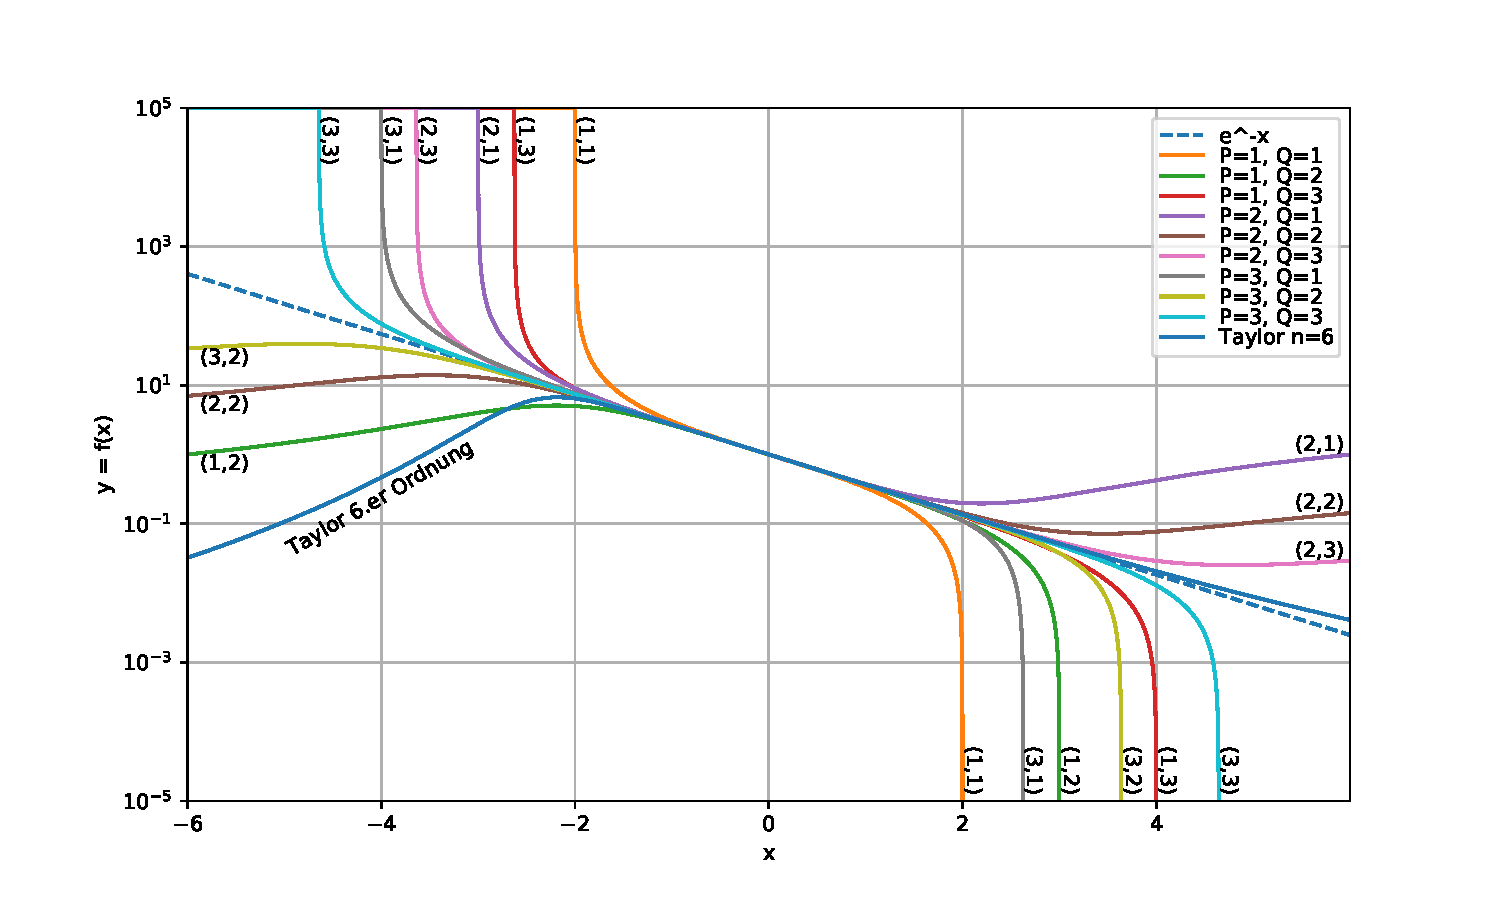
\includegraphics[width=1\linewidth]{./papers/pade/python/bilder/totzeit.pdf}
	\caption{Plot der Padé-Approximanten der Exponentialfunktion im Vergleich zu der Originalfunktion in einer logarithmischen Skala vergleichend mit der Taylor-Reihe sechster Ordnung der Exponentialfunktion.\label{pade:totzeitexp}}
\end{figure}

Die Grade werden dabei im Nenner und Zähler unterteilt aufgezeigt.
Im Beispiel \ref{pade:totzeitexp} mit der Exponentialfunktion, erweisen sich die Polynome des selben Grades im Nenner und Zähler als die genauesten Approximationen.
Wobei mit steigendem Grad der Approximation eine stetige Verbesserung erzielt wird.
Zum Vergleich wurde noch die Taylor-Reihe von $e^{-x}$ der sechsten Ordnung in der Grafik \ref{pade:totzeitexp} dargestellt. 
Diese ist im negativen Bereich der Funktionsachse deutlich schlechter als die Padé-Approximanten, jedoch verhält sie sich im positiven Bereich besser.


Nehmen wir nun diese Polynome, welche sich noch im Frequenzbereich befinden und transformieren diese wieder zurück in den Zeitbereich, erhalten wir die in der Grafik \ref{pade:totzeitexp2} dargestellten Kurven.

\begin{figure}[!h]
	\centering
	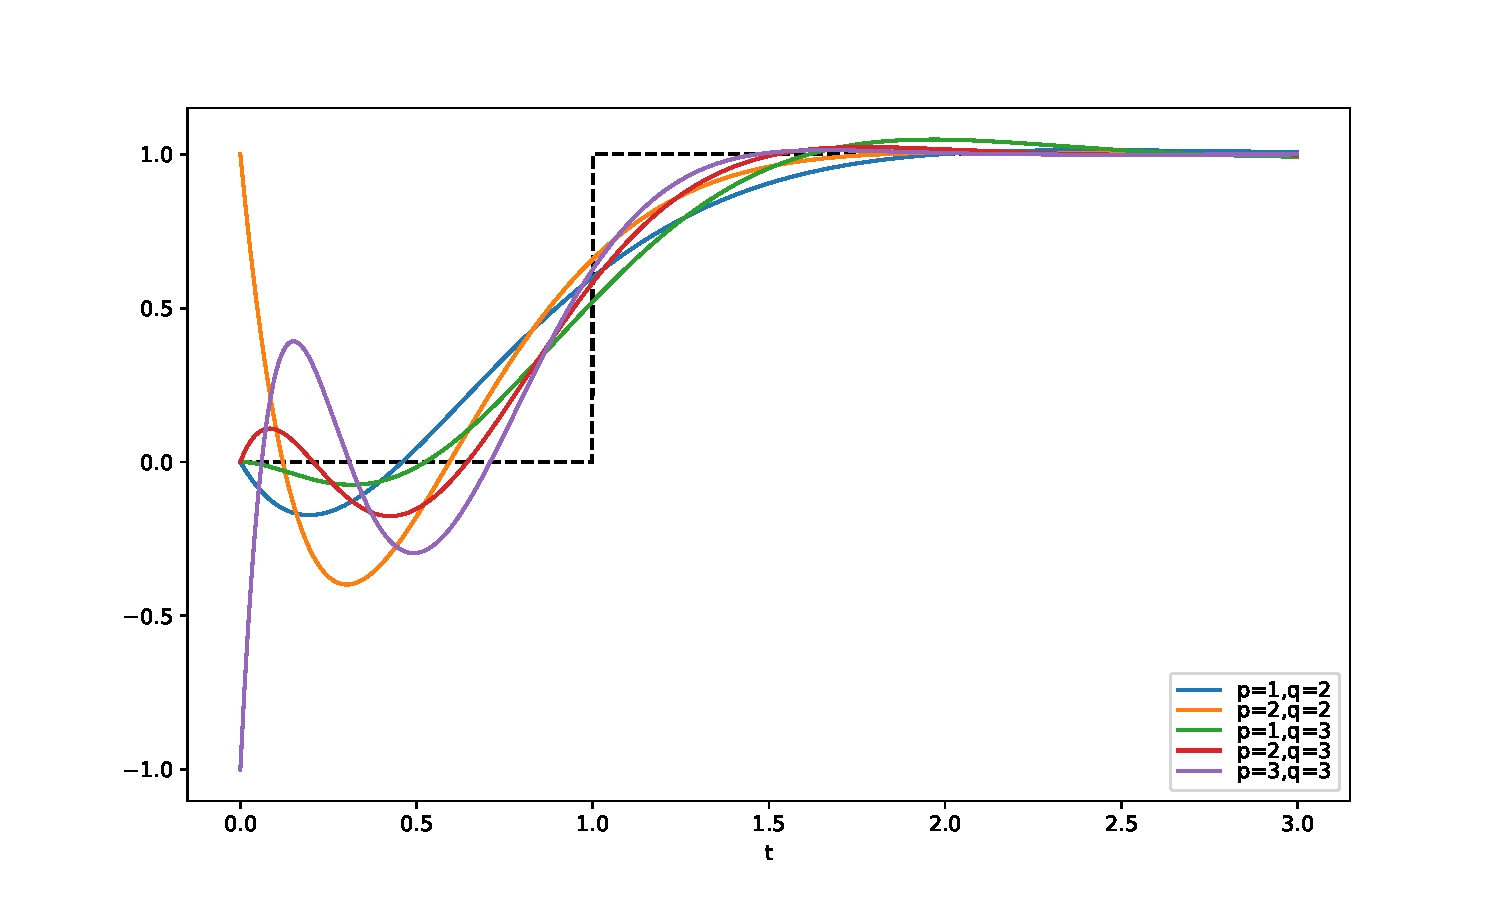
\includegraphics[width=1\linewidth]{./papers/pade/python/bilder/padelow33.pdf}
	\caption{In den Zeitbereich zurück transformierte Polynome tieferer Ordnung\label{pade:totzeitexp2}.}
\end{figure}

Die Polynome unterer Ordnung sind dabei noch weit von einem brauchbaren Ergebnis des gesuchten verzögerten Einheitssprunges entfernt.
Man kann nun die Ordnung der Polynome weiter erhöhen bis man eine zufriedenstellende Approximation erhält.
Dabei muss man jedoch aufpassen welche Methode für die Rücktransformation verwendet wird.
Nicht alle Implementationen der Rücktransformation von Übertragungsfunktionen in ein Zustandsraummodell sind nummerisch stabil. 
Bei Polynomen grosser Ordnung oder wenn das Nenner- und Zähler- Polynom nicht gleicher Ordnung sind, können bei einer Rücktarnformation Fehler auftauchen.
Dies ist jedoch ein anderes Thema, welches den Rahmen dieses Papers sprengen würde und wird deshalb nicht weiter beschrieben.


\begin{figure}[h]
	\centering
	\subfigure[Pole und Nullstellen im Bildbereich geplottet wenn $P=Q$ ist.\label{pade:poles1}]{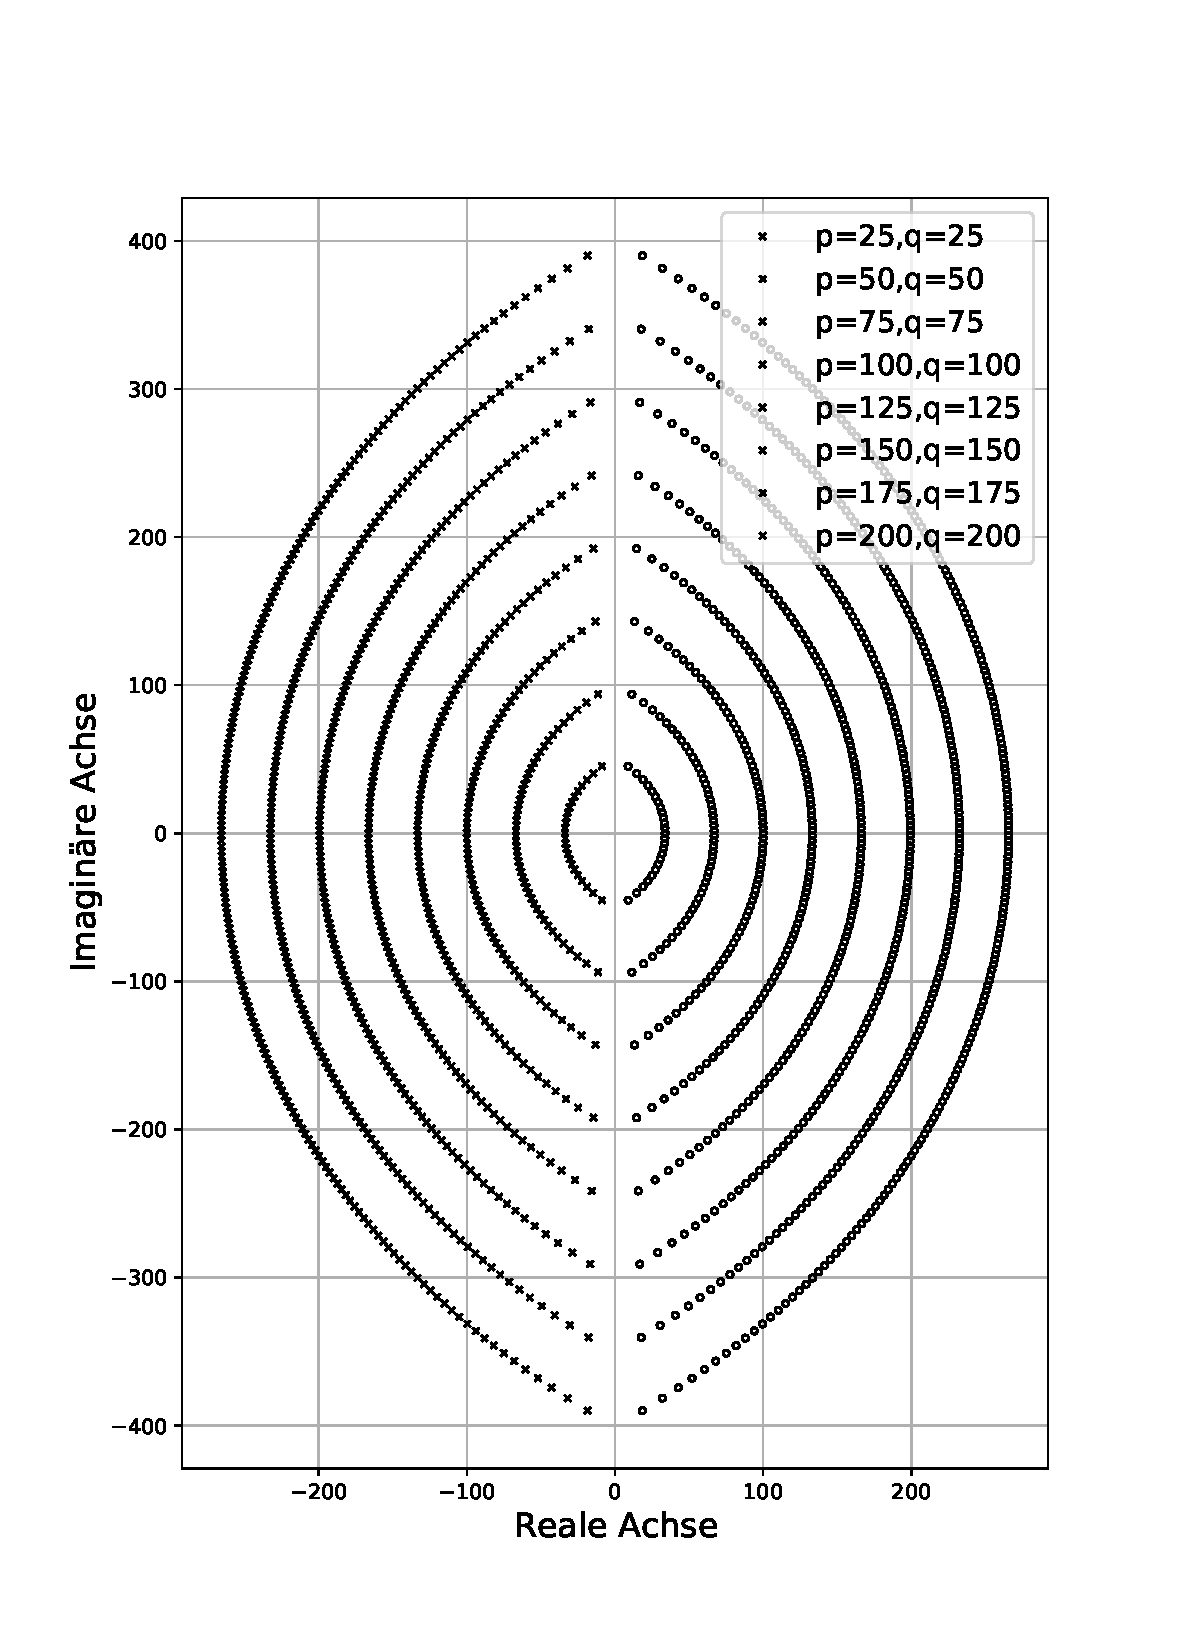
\includegraphics[width=0.40\linewidth]{./papers/pade/python/bilder/poles1.pdf}}
	\subfigure[Pole und Nullstellen im Bildbereich geplottet wenn $P>Q$ ist.\label{pade:poles2}]{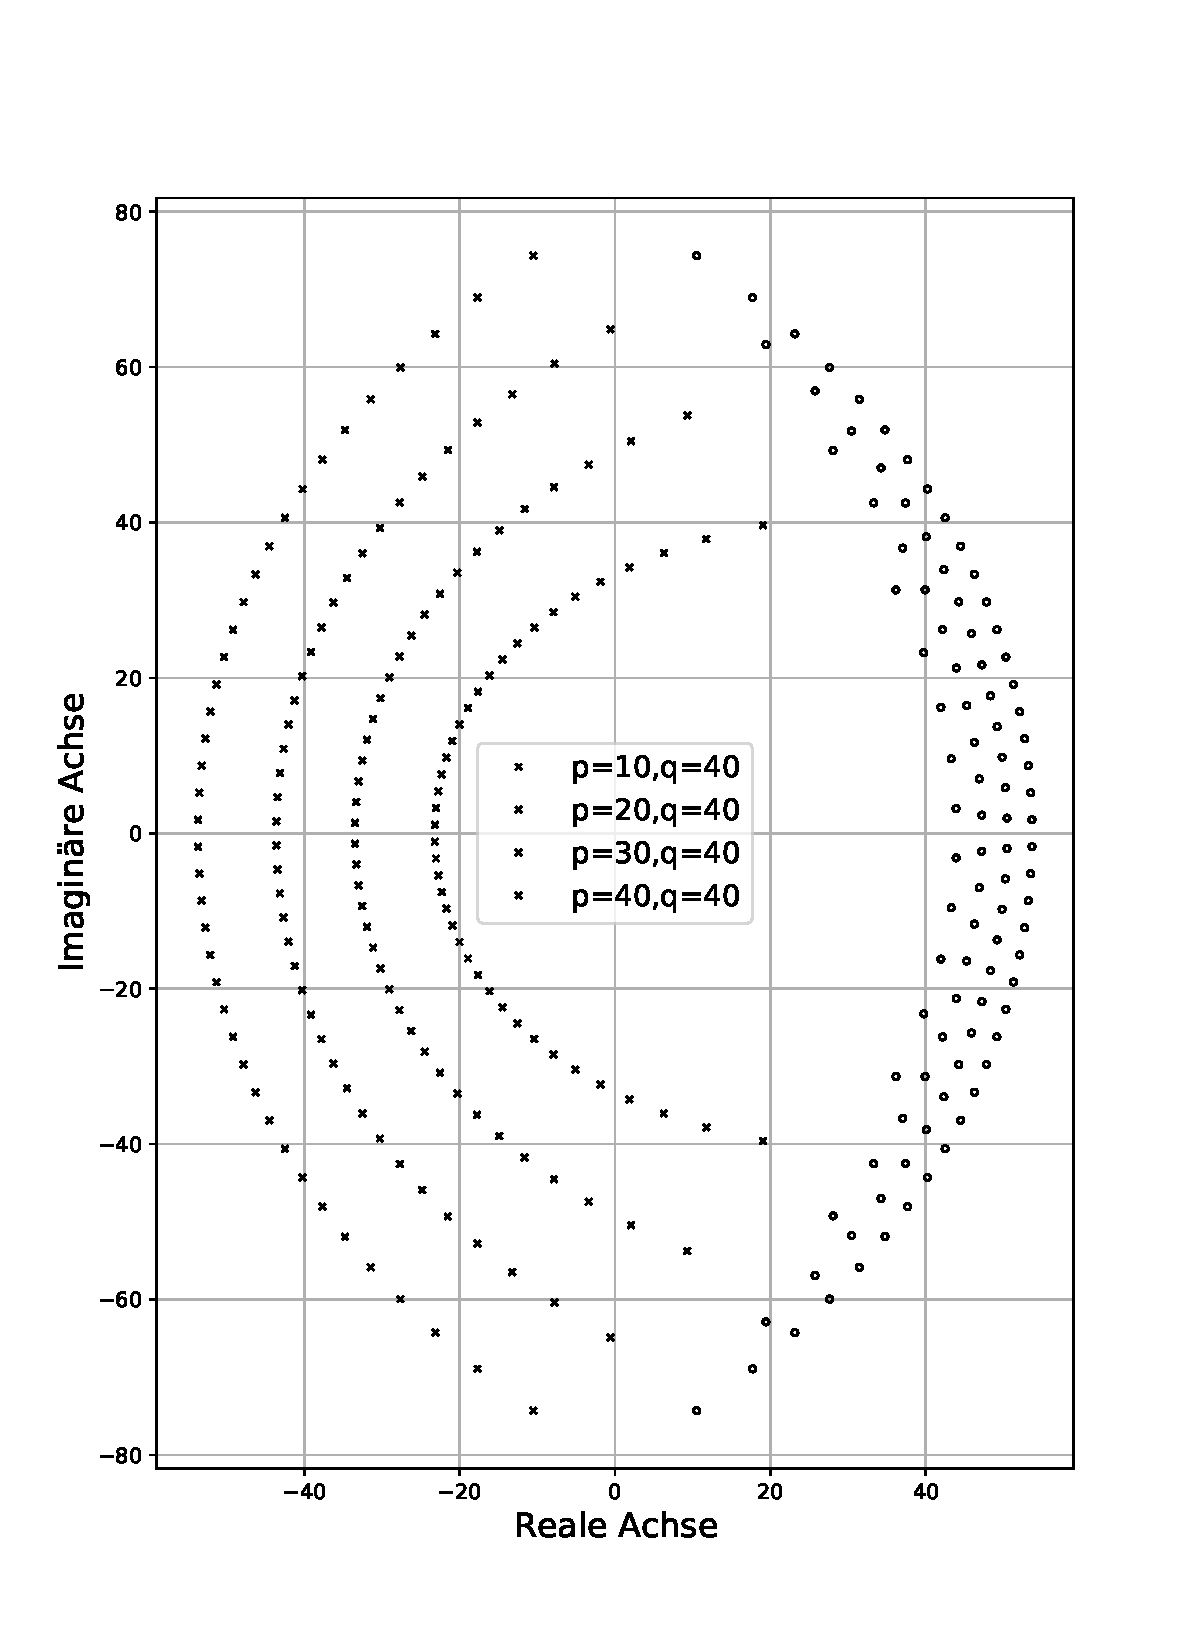
\includegraphics[width=0.40\linewidth]{./papers/pade/python/bilder/poles2.pdf}}
	\subfigure[Pole und Nullstellen im Bildbereich geplottet wenn $P<Q$ ist.\label{pade:poles3}]{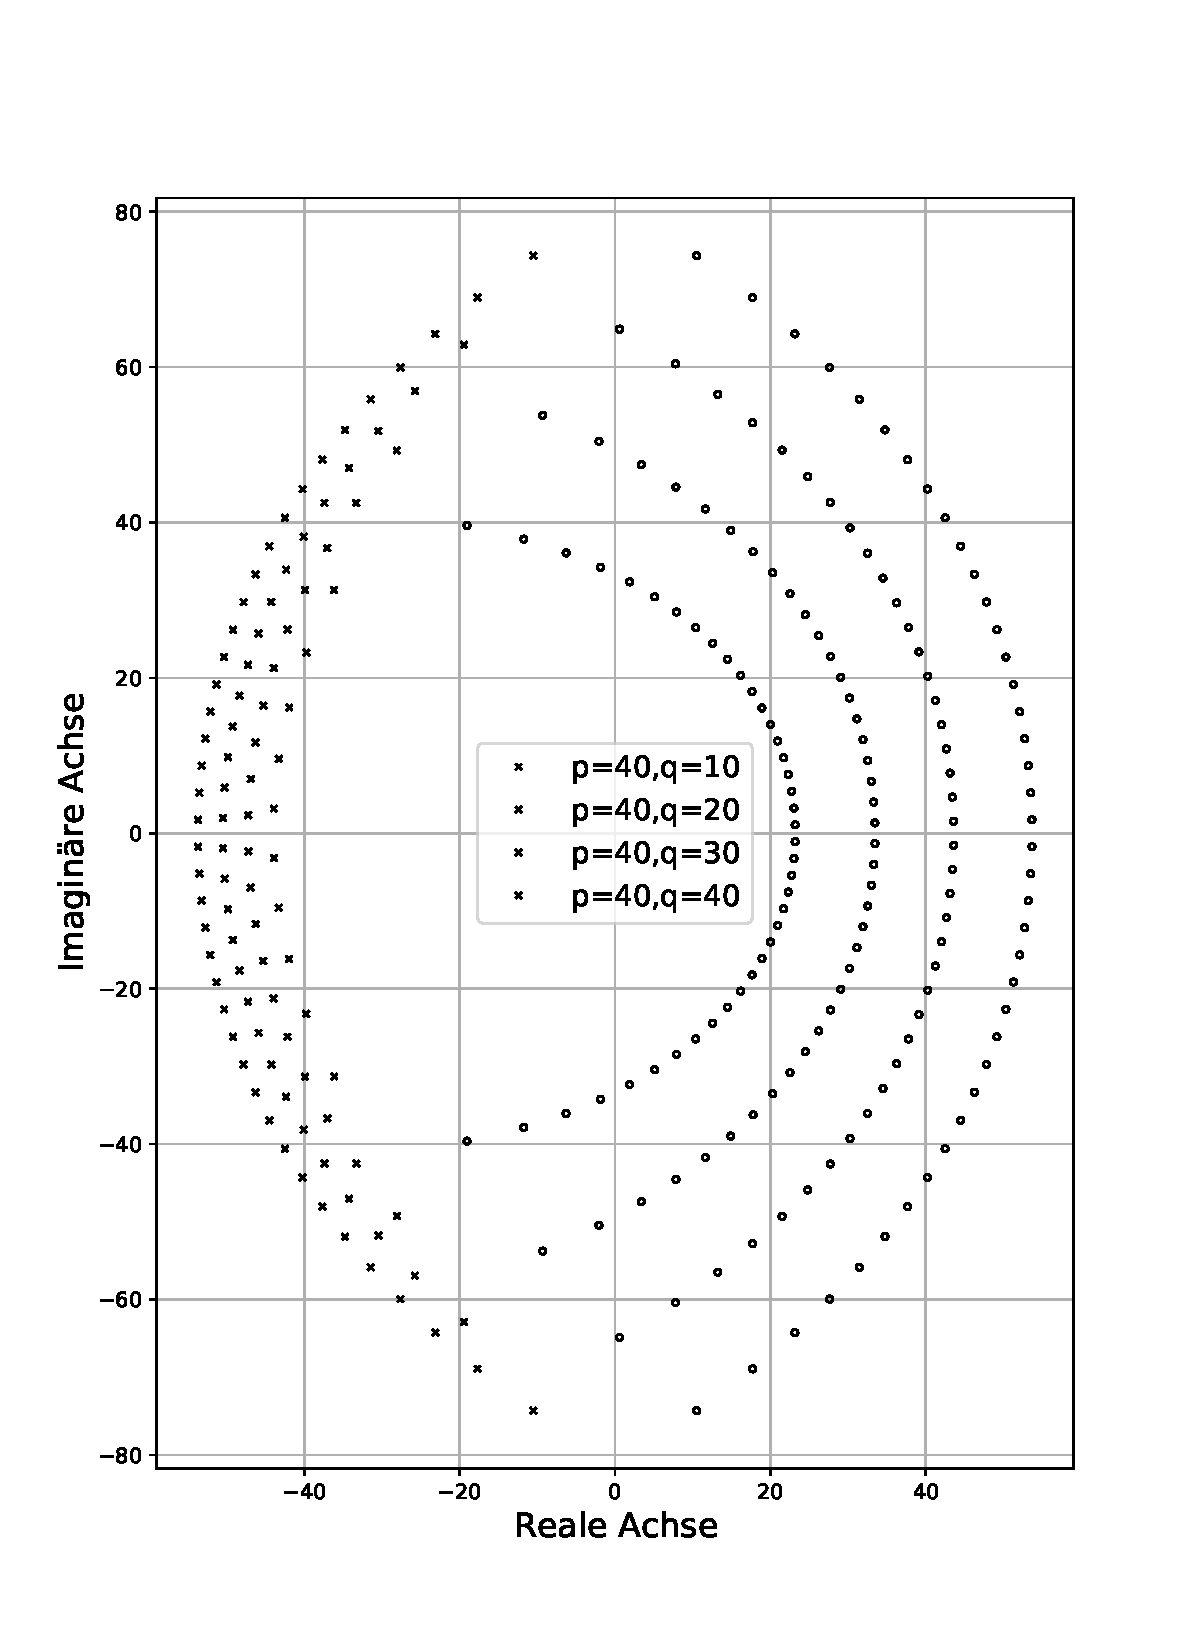
\includegraphics[width=0.40\linewidth]{./papers/pade/python/bilder/poles3.pdf}}
	\caption{Visualisierung der Stabilität der Padé-Polynome bei ungleicher $[L/M]$ Ordnung. \label{pade:prole}}
\end{figure}

In der Grafik \ref{pade:prole} sind nun die Pol- und Nullstellen von höheren Ordnungen dargestellt. 
Auffallend ist die schöne Symmetrie der Pol- und Nullstellen welche bei gleicher Ordnung der Nenner- und Zähler- Polynome um den Nullpunkt verteilt sind.
Diese Symmetrie verschwindet wenn der Grad des Nenner- oder des Zähler- Polynoms grösser gewählt wird.
Dies kann man soweit treiben, bis eine Polstelle in den rechten Bereich der komplexen Halbebenen reicht \ref{pade:poles2},
was ein instabiles System zur folge hat.
Ein instabiles System beutetet hier, dass der rücktransformierte Einheitssprung eine immer grösser werdende Schwingung ist.
 
\begin{figure}
	\centering
	\subfigure[Pole und Nullstellen im Bildbereich geplottet wenn $P=Q$ ist.\label{pade:totzeit1}]{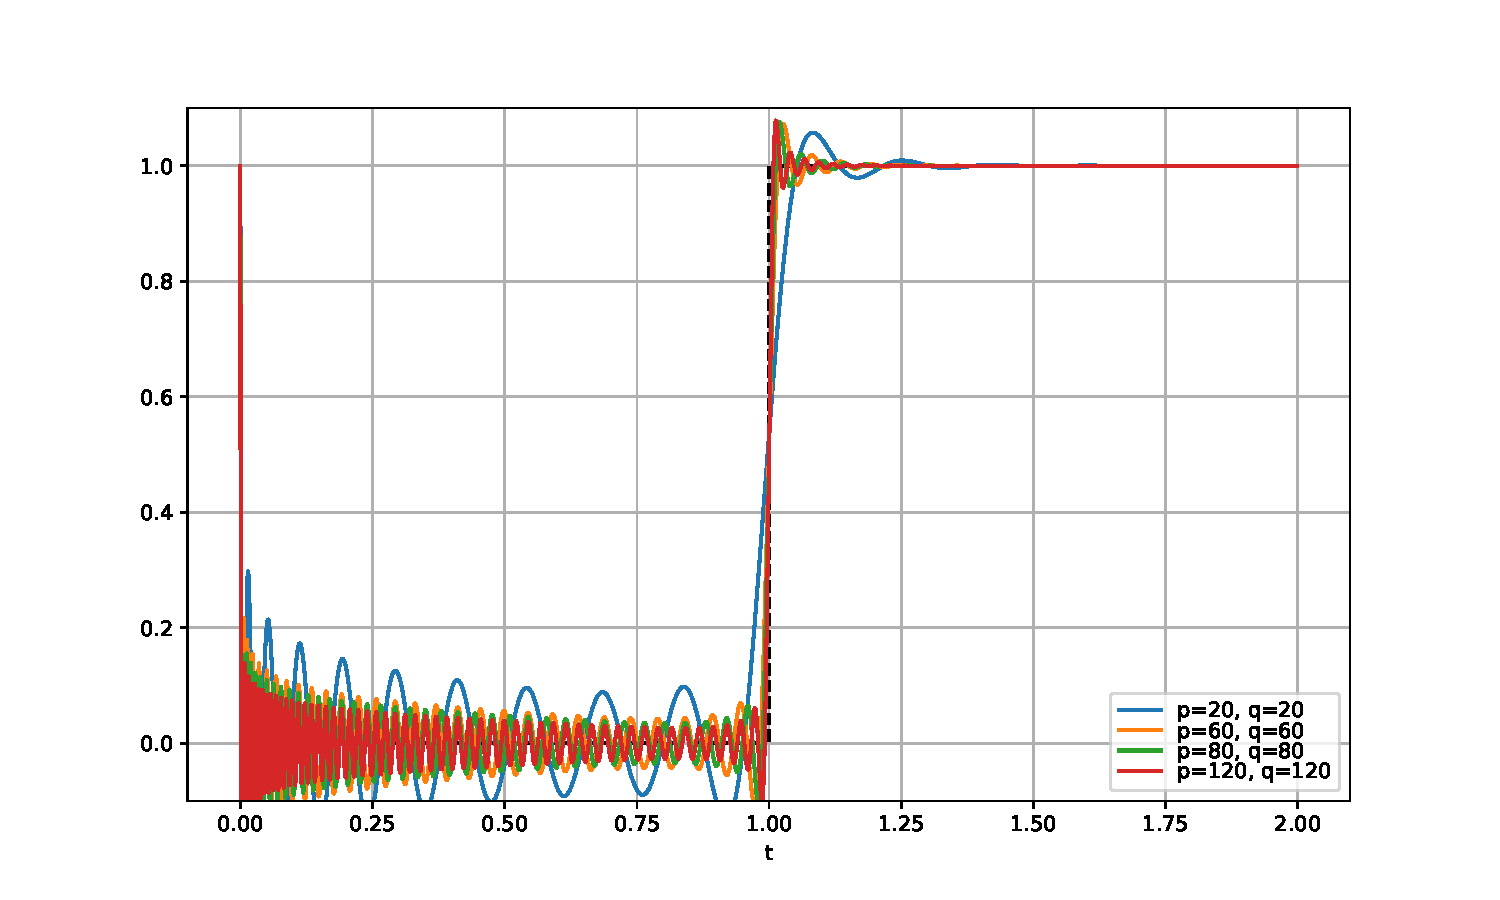
\includegraphics[width=1\linewidth]{./papers/pade/python/bilder/padehigh1.pdf}}
	\subfigure[Pole und Nullstellen im Bildbereich geplottet wenn $P=Q-10$ ist.\label{pade:totzeit2}]{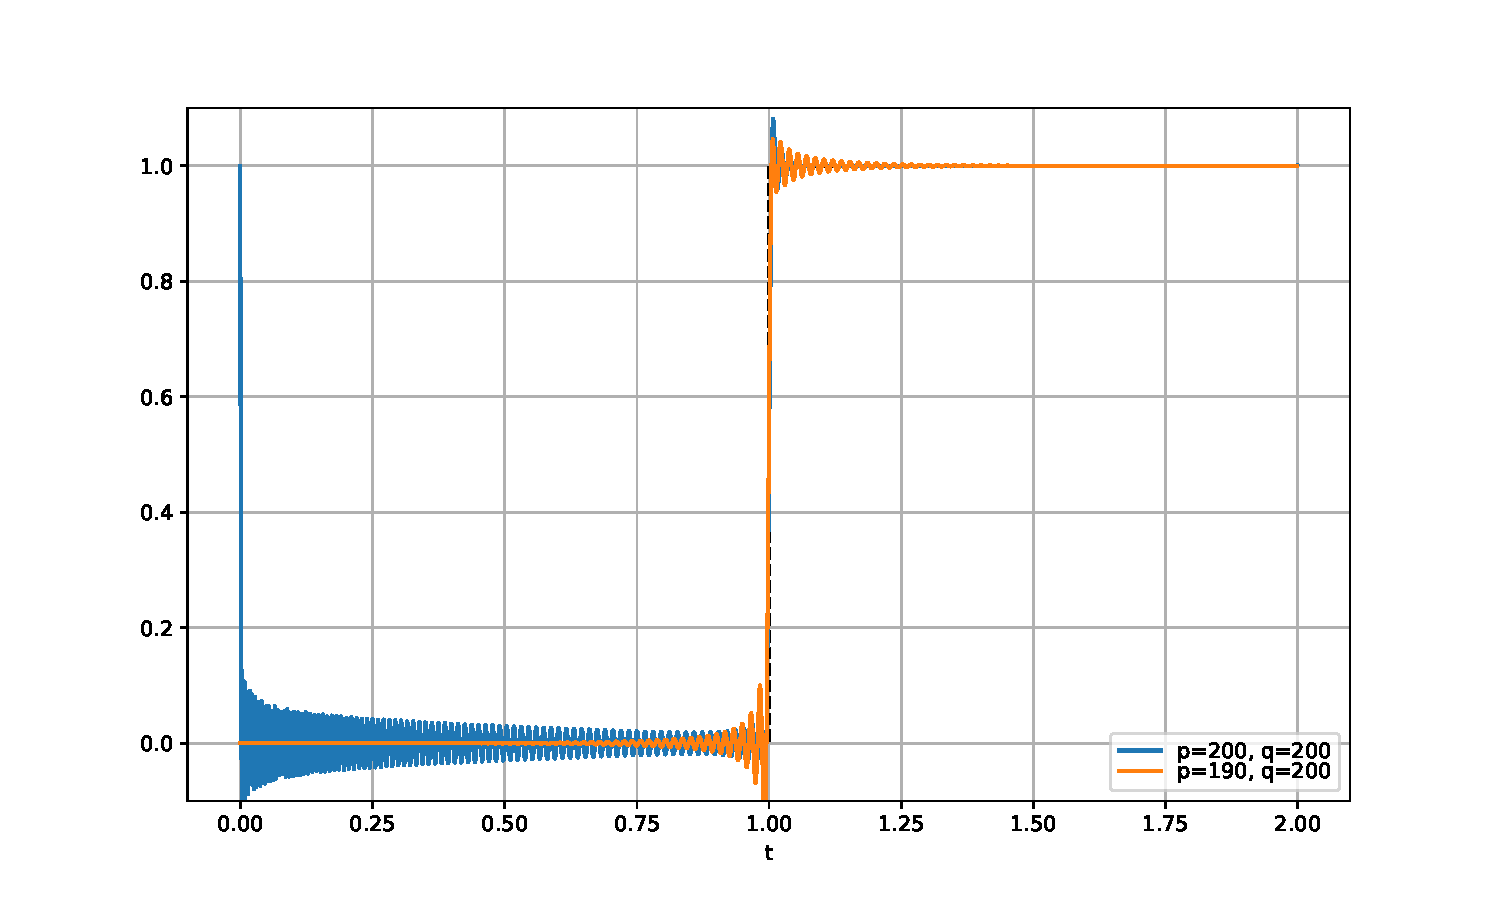
\includegraphics[width=1\linewidth]{./papers/pade/python/bilder/padehigh2.pdf}}
\end{figure}
Verwendet man nun die Approximanten höherer und gleicher Ordnung für die Rücktransformation in Grafik \ref{pade:totzeit1}, erhält man einen immer besser werdenden Einheitssprung mit einem kleinen Überschwinger vor und nach dem Sprung. 
Auffallend ist hier, dass der Padé-Approximant höchster Ordnung zu beginn den grössten Fehlerpeak hat.
Dieser ist sogar so hoch wie der Einheitssprung selbst.

Um diesen Fehlerpeak zu Beginn ein wenig zu vermindern, können nun die Pole in der komplexen Ebene ein wenig näher zur positiven Halbebene gebracht werden.
Wie schon in  dem Pol- Nullstellendiagramm \ref{pade:poles2} erkennbar, ist das mit einer Differenz von der Ordnung des Zählerpolynoms $p$ und Nennerpolynom $q$ möglich.
Mit einer Differenz von 190 zu 200 der Polynom Ordnung wurde die Rücktransformierte des Padé-Approximanten der Grafik \ref{pade:totzeit2} dargestellt.
Deutlich zu sehen ist dabei, dass der Überschwinger, welcher bei dem Padé-Approximanten gleicher Ordnung in derselben Grafik \ref{pade:totzeit2} noch vorhanden ist, verschwindet.
Jedoch besitzt der Approximant ungleicher Ordnung eine längere Einschwingzeit als der mit gleicher Ordnung. 
Mit diesen Werten der Ordnungen kann in der Praxis solange optimiert werden, bis man die beste Lösung für sein Problem gefunden hat.
Es gäbe dabei noch die Möglichkeit, weitere Filter einzubauen, um diese Schwingungen zu dämpfen und ein noch besseres Resultat zu erzielen.


\newpage

\subsection{Signal Modellierung
	\label{pade:subsection:SignalMod}}

Das Ziel einer Signalmodellierung ist, dass eine parametrische Beschreibung eines Signales gefunden wird.
Dies kann für die Filterentwicklung, Interpolation, Extrapolation oder Kompression verwendet werden.
Dabei kann man immer das gleiche Modell verwenden, welches der Ausgang $x(n)$ eines linearen verschiebungsinvarianten Filters zu einem Eingang $v(n)$ darstellt. 
 
\begin{center}
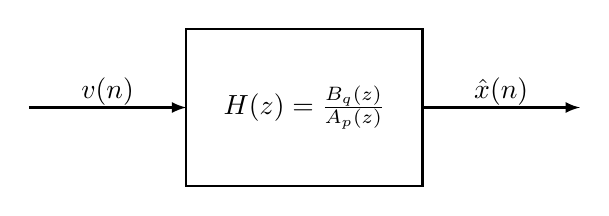
\begin{tikzpicture}
\tikzset{>=latex}
\node at (-1,1.2)  {$v(n)$}; 
\draw[thick,->] (-2,1)--(0,1);
\draw[thick] (0,0) rectangle (3,2) node[pos=.5] {$H(z)=\frac{B_q (z)}{A_p (z)}$};
\draw[thick,->] (3,1)--(5,1);
\node at (4,1.2)  {$\hat{x}(n)$}; 
\end{tikzpicture}
\end{center}

Dieses Modell wird mit
\begin{equation}
H(z)
=
\frac{B_{q}(z)}{A_{p}(z)}
=
\frac{\sum_{k=0}^{q} b_{q}(k) z^{-k}}{1+\sum_{k=1}^{p} a_{p}(k) z^{-k}}
\end{equation}
als eine rationale Funktion beschrieben.
Das Ziel ist es einen Filter $H(z)$ und ein Input $v(n)$, welche $\hat{x}(n)$ so nahe wie möglich an $x(n)$ bringen, zu finden.
Das Eingangssignal, welches auf den Filter wirkt, ist meist ein diskreter Impuls $\delta(n)$.
Der Modellierungsfehler $e^{\prime}(n)$ setzt sich aus der Differenz der Einheitssprungantwort $h(n)$ und dem diskreten Signal $x(n)$ zusammen.
\begin{center}
	\tikzset{>=latex}
	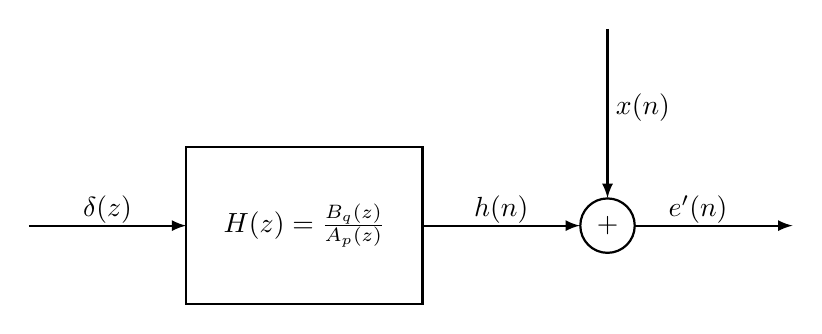
\begin{tikzpicture}
	\node at (-1,1.2)  {$\delta(z)$}; 
	\draw[thick,->] (-2,1)--(0,1);
	\draw[thick] (0,0) rectangle (3,2) node[pos=.5] {$H(z)=\frac{B_q (z)}{A_p (z)}$};
	\draw[thick,->] (3,1)--(5,1);
	\node [circle, draw, thick] at (5.35,1){+};
	\draw[thick,->] (5.35,3.5)--(5.35,1.35);
	\draw[thick,->] (5.7,1)--(7.7,1);
	\node at (4,1.2)  {$h(n)$}; 
	\node at (5.8,2.5)  {$x(n)$}; 
	\node at (6.5,1.2)  {$e^{\prime}(n)$}; 
	\end{tikzpicture}
\end{center}
Ziel ist es den quadratischen Fehler 
\begin{equation}
E_{L S}
=
\sum_{n=0}^{\infty}\left|e^{\prime}(n)\right|^{2}
\end{equation}
des Systems zu minimieren (Least Squares Method).
Um dies zu erreichen, werden die Ableitungen   
\begin{equation}\begin{array}{ll}
\frac{\partial E_{L S}}{\partial a_{p}^{*}(k)}
=
0 
& 
\text{mit } k=1,2, \ldots, p \\
&\\

\frac{\partial E_{L S}}{\partial b_{q}^{*}(k)}
=
0  
&
 \text{mit } k=0,1, \ldots, q
\end{array}\end{equation}
gleich 0 gesetzt.
Aus diesen Bedienungen resultiert eine Menge von nichtlinearen Gleichungen 

\begin{align*}
\frac{\partial E_{L S}}{\partial a_{q}^{*}(k)}
&=
\frac{1}{2 \pi} 
\int_{-\pi}^{\pi}
\left[X\left(e^{j \omega}\right)-\frac{B_{q}\left(e^{j \omega}\right)}{A_{p}\left(e^{j \omega}\right)}\right] 
\frac{B_{q}^{*}\left(e^{j \omega}\right)}{A_{p}^{*}\left(e^{j \omega}\right)^{2}} 
e^{j k \omega} d \omega
=
0\\
\frac{\partial E_{L S}}{\partial b_{q}^{*}(k)}
&=
-\frac{1}{2 \pi} 
\int_{-\pi}^{\pi}
\left[X\left(e^{j \omega}\right)-\frac{B_{q}\left(e^{j \omega}\right)}{A_{p}\left(e^{j \omega}\right)}\right] 
\frac{e^{j k \omega}}{A_{p}^{*}\left(e^{j \omega}\right)} d \omega
=
0
\end{align*}
welche möglicherweise sehr schwierig lösbar sind.
Aus diesem Grund wird in der Praxis der Ansatz des kleinsten quadratischen Fehlers vermieden. 
Um diese nichtlinearen Gleichungen zu vermeiden und dennoch eine Lösung zu finden, welche uns eine passende Anzahl von $x[n]$ Werten mit der Einheitssprungantwort verbindet, kann ein eleganter Trick, der zur Padé-Approximation führt verwendend werden. 
\begin{equation}
H(z) A_{p}(z)=B_{q}(z)
\end{equation}
In der Zeitebene betrachtet handelt es sich in bei dieser Gleichung um eine Faltung.
\begin{equation}
h(n)+\sum_{k=1}^{p} a_{p}(k) h(n-k)=b_{q}(n)
\end{equation}
Die rechte Seite der Gleichung für $n>q$ ist dabei gleich null.
Diese Fallunterscheidung
\begin{equation}
x(n)+\sum_{k=1}^{p} a_{p}(k) x(n-k)
=
\left\{\begin{array}{cc}
b_{q}(n) & 
\quad \text{mit } \quad n=0,1, \ldots, q \\
0 & 
\quad \quad \quad\text{mit } \quad n=q+1, \ldots, q+p
\end{array}\right.\end{equation}
kann in die Matrixform 
\begin{equation}
\left[\begin{array}{cccc}
x(0) & 0 & \cdots & 0 \\
x(1) & x(0) & \cdots & 0 \\
x(2) & x(1) & \cdots & 0 \\
\vdots & \vdots & & \vdots \\
x(q) & x(q-1) & \cdots & x(q-p) \\
x(q+1) & x(q) & \cdots & x(q-p+1) \\
\vdots & \vdots & & \vdots \\
x(q+p) & x(q+p-1) & \cdots & x(q)
\end{array}\right]
\left[\begin{array}{c}
1 \\
a_{p}(1) \\
a_{p}(2) \\
\vdots \\
a_{p}(p) \\
\end{array}\right]
=
\left[\begin{array}{c}
b_{q}(0) \\
b_{q}(1) \\
b_{q}(2) \\
\vdots \\
b_{q}(q) \\
0 \\
\vdots \\
0
\end{array}\right]
\end{equation}
gebracht werden.
Diese Matrix ist uns schon aus dem Abschnitt \ref{pade:subsection:Pade_erstellen} bekannt. Es handelt sich nämlich um eine Padé-Approximation,
welche wir nun für das Signal mit einer vorgegebener Ordnung berechnen können.

\begin{beispiel}

Die ersten sechs Signale eines Signales sind vorgegeben.
\begin{equation*}
\bm x=\left[
\begin{array}{l}
1.0000\\
1.5000\\
0.7500\\
0.3750\\
0.1875 \\
0.0938
\end{array}\right]
\end{equation*}
Das Ziel ist drei verschiedene Padé-Approximanten mit drei verschiedenen Freiheitsgraden zu finden.
\begin{equation*}\begin{aligned}
&\begin{array}{ll}
\text { All pole } & (q=0, p=2) \\
\text { FIR } & (q=2, p=0)\\
\text { IIR } &(\mathrm{q}=1, \mathrm{p}=1)
\end{array}\\
\end{aligned}\end{equation*}

Das All pole Modell $(q=0,p=2)$ wird in die Matrixform
\begin{equation}\left[\begin{array}{ccc}
x(0) & 0 & 0 \\
x(1) & x(0) & 0 \\
x(2) & x(1) & x(0)
\end{array}\right]\left[\begin{array}{c}
1 \\
a_1 \\
a_2
\end{array}\right]=\left[\begin{array}{c}
b_0 \\
0 \\
0
\end{array}\right]\end{equation}
gebracht. 
Von der ersten Gleichung folgt, dass der Wert $b_0 = x(0)=1$ ergeben muss. 
Weiter können nun die letzten zwei Gleichungen
\begin{equation}\left[\begin{array}{ll}
x(0) & 0 \\
x(1) & x(0)
\end{array}\right]\left[\begin{array}{l}
a_1 \\
a_2
\end{array}\right]=-\left[\begin{array}{l}
x(1) \\
x(2)
\end{array}\right]\end{equation}
eingesetzt und gelöst werden.
\begin{equation}\left[\begin{array}{cc}
1 & 0 \\
1.5 & 1
\end{array}\right]\left[\begin{array}{l}
a_1 \\
a_2
\end{array}\right]=-\left[\begin{array}{c}
1.50 \\
0.75
\end{array}\right]\end{equation}
\begin{equation}
a_1=-1.50 \quad  \quad a_2=1.50
\end{equation}

Somit haben wir das Ergebnis für unser $x(n)$ 
\begin{equation}
H(z)=\frac{1}{1-1.50 z^{-1}+1.50 z^{-2}}
\end{equation}
berechnet.
Man sollte beachten, dass sich die Pole nicht im Einheitskreis befinden und somit das Resultat kein stabiles Modell sein wird.

Für das FIR-Modell $(q=2,P=0)$ ist das Resultat einfach mit $A(z)=1$ berechenbar.

\begin{equation}\begin{array}{r}

{\left[\begin{array}{l}
	x(0) \\
	x(1) \\
	x(2)
\end{array}\right]
=
\left[\begin{array}{l}
	b_0 \\
	b_1 \\
	b_2
	\end{array}\right]}
\end{array}\end{equation} 
Somit erhalten wir 
\begin{equation}
H(z)=1+1.50 z^{-1}+0.75 z^{-2}
\end{equation}
als unser Modell.

Für das IIR-Modell mit $(q=1,p=1)$ welches die Form
\begin{equation}
H(z)=\frac{b(0)+b(1) z^{-1}}{1+a(1) z^{-1}}
\end{equation}
erhalten wird, sind die Padé-Gleichungen

\begin{equation}\left[\begin{array}{ll}
x(0) & 0 \\
x(1) & x(0) \\
x(2) & x(1)
\end{array}\right]\left[\begin{array}{c}
1 \\
a_1
\end{array}\right]=\left[\begin{array}{c}
b_0 \\
b_1\\
0.
\end{array}\right]\end{equation}
Der Pol in der letzten Gleichung 
\begin{equation}
x(2)+a_1 x(1)=0
\end{equation}
kann damit gerechnet werden.
Eingesetzt und nach $a_1$ aufgelöst erhalten wir
\begin{equation}
a_1=-\frac{x(2)}{x(1)}=
-\frac{0.75}{1.5}=
-0.5.
\end{equation}
Mit den bekannten Polen können nun die Nullstellen mit den oberen zwei Gleichungen 
\begin{equation}\left[\begin{array}{c}
b_0 \\
b_1
\end{array}\right]=\left[\begin{array}{cc}
1 & 0 \\
1.5 & 1
\end{array}\right]\left[\begin{array}{c}
1 \\
-0.5
\end{array}\right]=\left[\begin{array}{l}
1 \\
1
\end{array}\right]\end{equation}
berechnet werden.
Die Koeffizienten können nun in das Modell eingesetzt werden, womit wir
\begin{equation}
H(z)=\frac{1+z^{-1}}{1-0.5 z^{-1}}
\end{equation}
erhalten.
Dieses Modell hat eine identische Einheitssprungantwort 
\begin{equation}
h(n)=(0.5)^{n} u(n)+(0.5)^{n-1} u(n-1)
=
\delta(n)+1.5(0.5)^{n-1} u(n-1)\end{equation}
wie $x(n)$.
Dies ist jedoch ein Spezialfall und kommt nicht immer vor.
\end{beispiel}







%
% problemstellung.tex -- Beispiel-File für die Beschreibung des Problems
%
% (c) 2020 Prof Dr Andreas Müller, Hochschule Rapperswil
%
\section{Folgerungen
\label{quadratur:section:folgerungen}}
\rhead{Folgerungen}

\subsection{Vergleich Gauss-Quadratur mit Trapezregel}
In diesem Abschnitt werden die Resultate der Gauss-Quadratur mit Resultaten der Trapezregel
verglichen, um zu zeigen wie effizient die Integration mit der Gausss-Integration ist.
Dazu wird nochmals die Funktion $\sqrt{1-x^{2}}$ Integriert. 
Die Resultate sind in der Tabelle~\ref{buch:table:gaussvergleich} dargestellt.
Als Referenz: Das analytische Resultat des Integrals ist $\frac{\pi}{2} \approx 1.5707963268$.
\begin{table}
    \centering
    \begin{tabular}{|>{$}c<{$}|>{$}c<{$}|>{$}c<{$}|>{$}c<{$}|>{$}c<{$}|}
        \hline
        n & \text{Gauss-Quadratur} &  \text{Gauss-Quadratur} & \text{Trapezregel} & \text{Trapezregel} \\
         & \text{Resultat} &  \text{Fehler} & \text{Resultat} & \text{Fehler} \\
        \hline  
        2 & 1.6329931619 & 0.3670068381 & 0.0000000000 & 1.5707963268 \\
        3 & 1.5916172578 & 0.0413759040 & 1.0000000000 & 0.5707963268 \\
        4 & 1.5802775277 & 0.0113397301 & 1.2570787221 & 0.3137176047 \\
        5 & 1.5759063349 & 0.0043711928 & 1.3660254038 & 0.2047709230 \\
        7 & 1.5727819554 & 0.0010820282 & 1.4587766894 & 0.1120196374 \\
        10 & 1.5715139556 & 0.0002531675 & 1.5096159164 & 0.0611804104 \\
        20 & 1.5708921460 & 1.55366 \cdot e^{-05} & 1.5507798233 & 0.020016503 \\
        30 & 1.5708253858 & 3.05870 \cdot e^{-06} & 1.5601695280 & 0.010626799 \\
        40 & 1.5708087326 & 9.66660 \cdot e^{-07} & 1.5639786384 & 0.006817688 \\
        50 & 1.5708027245 & 3.95730 \cdot e^{-07} & 1.5659537235 & 0.004842603 \\
        100 & 1.5707971383 & 2.47153 \cdot e^{-08} & 1.5691090196 & 0.001687307 \\
        \hline
    \end{tabular}
    \caption{Resultatvergleich zwischen der Gauss-Quadratur und der Trapezregel
\index{Resultatvergleich}
    \label{buch:table:gaussvergleich}}   
\end{table}
Man kann sehr schön sehen, dass die Resultate der Gauss-Quadratur mit nur wenigen Funktionsauswertungen
schon sehr geringe Abweichungen vom analytischen Resultat haben, während bei der Trapezregel
viel mehr Funktionsauswertungen benötigt werden, um die selbe Genauigkeit zu erreichen.
Man sieht, dass die Genauigkeit der Trapezregel mit $n = 100$ bei der Gauss-Quadratur bereits mit $n = 7$
erreicht wird.

\subsection{Programm für Gauss-Quadratur in Python}
\index{Python}%
In Python lässt sich die Gauss-Quadratur in gerade mal $25$ Zeilen Code umsetzen.
Dafür wird aus dem Modul \texttt{scipy} die Klasse \texttt{integrate} importiert. 
Ausserdem wird für die mathematischen Funktionen das Modul \texttt{numpy} verwendet
\index{numpy@\texttt{numpy}}
\begin{lstlisting}[float,language=Python,style=Python]
    import numpy as np
    from scipy import integrate

    # Warnungen werden erzeugt, wenn mit der gewaehlten Anzahl
    # Stuetzstellen die Toleranz  tol=1.49e-08 nicht erreicht werden kann

    # Zu integrierende Funktion
    func = lambda x: np.sqrt(1 - x ** 2)

    # Anzahl Stuetzstellen in einem Array. 
    nodes = [1, 2, 3, 4, 5, 7, 10, 20, 30, 40, 50, 100]

    # Quadraturen mit node = Anzahl Stuetzstellen
    for node in nodes:
        x = np.linspace(-1, 1, node)
        y = func(x)
        print(f"Number of nodes: {node}")
        # Berechnung mit Gauss-Quadratur
        print(f"Gauss-Legendre : {integrate.quadrature(func, -1, 1, maxiter=node)}")
        # Berechnung mit Trapezformel
        trapez = integrate.trapz(y, x)
        print(f"Trapezoidal Rule: {trapez}")
        # Berechnung mit Simpsonscher Regel
        print(f"Simpson's Rule : {integrate.simps(y, x)}")
        print()
\end{lstlisting}


\subsection{Fazit}
Die Gauss-Quadratur ist ein numerisches Integrationsverfahren, welches
mit wenigen Funktionsauswertungen das bestimmte Integral von beliebigen
Funktionen sehr genau berechnen kann. 
Polynome oder Annäherungen von Funktionen mittels Polynomen lassen sich 
sogar exakt berechnen und benötigen für ein Polynom vom Grad $2n+1$ nur 
$n$ Funktionsauswertungen.

Es gibt verschiedene Wege für die Bestimmung der Stützstellen und Gewichte.
Vorgerechnete Werte für $x_{i}$ und $A_{i}$ sind für grosse $n$ in Tabellen
vorhanden und erlauben schnelle Lookups. Für grössere $n$ existieren
Formeln, die die Berechnung der Stützstellen und Gewichte erlauben und
in Computerprogrammen einfach umgesetzt werden können.
Für verschiedene Integralgrenzen gibt es eigene Formen der Gauss-Quadratur
die auf orthogonalen Polynomen aufbauen, deren Nullstellen die Stützstellen
bestimmen.









\printbibliography[heading=subbibliography]
\end{refsection}
